\section{Software Solutions}\label{soft_sys_sec}

The software systems consist of three projects: pyroboime (AI), ssl-webclient
(graphical client), grSim (simulator).

\subsection{Artificial Intelligence}
% TODO: update software reestructure

The AI, pyroboime, is based on the STP (Skill-Tactic-Play) architecture and
implemented in python.
It has the following components: interface with the ssl-vision, ssl-refbox and
grSim, it also has a built-in communication module for the radio transmitter
system.
%The block diagram of the AI software is presented in figure \ref{fluxogramSoftware}.

The STP is a three tier architecture where the lowest level, skills, enables
the low level manipulations on a single robot.
The middle layer, tactics, makes use of the skill layer to execute higher level
behaviour, possibly enabling coopration, but still acting on a single robot.
The upper layer, plays, coordinates the tactics associated to each robot in
order to maximize performance, each play is implemented to behave according to
specific states: stop, halt, indirect kicks and normal play.
A higher level layer implmented as a play switches between other plays based on
the current referee state.
This architecture is better depicted in figure~\ref{fig:stp}.

\begin{figure}[H]
     \centering
     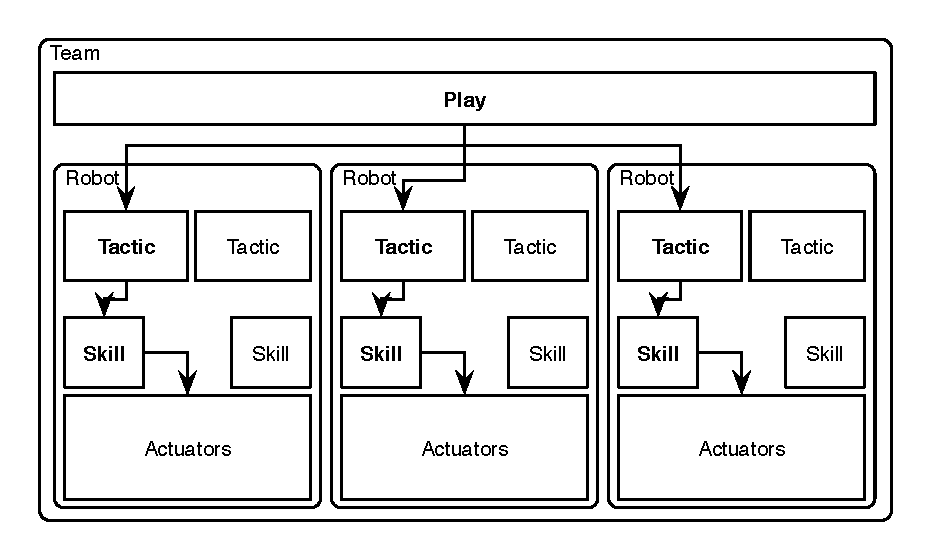
\includegraphics[width = \linewidth]{stp}
     \caption{STP Diagram}
     \label{fig:stp}
\end{figure}

There is also a skill implemented to redirect inputs from a joystick such that
it is possible to test the robot with little effort.

The interface is structured as a filter stack which connects the AI to a
flexible collection of updaters (which receive state information) and
commanders (which deliver commands to the robots, in both the simulated and
real environments).
It abstracts the external environment where the game is played from the AI\@.
Among the filters in said stack is a Kalman filter that reduces the noise
comming from the updater data.

The built-in radio trasmitter system interfaces with libusb to control the transmitter hardware, which is connected via USB.

%\begin{landscape}
%\begin{figure}[H]
%     \centering
%     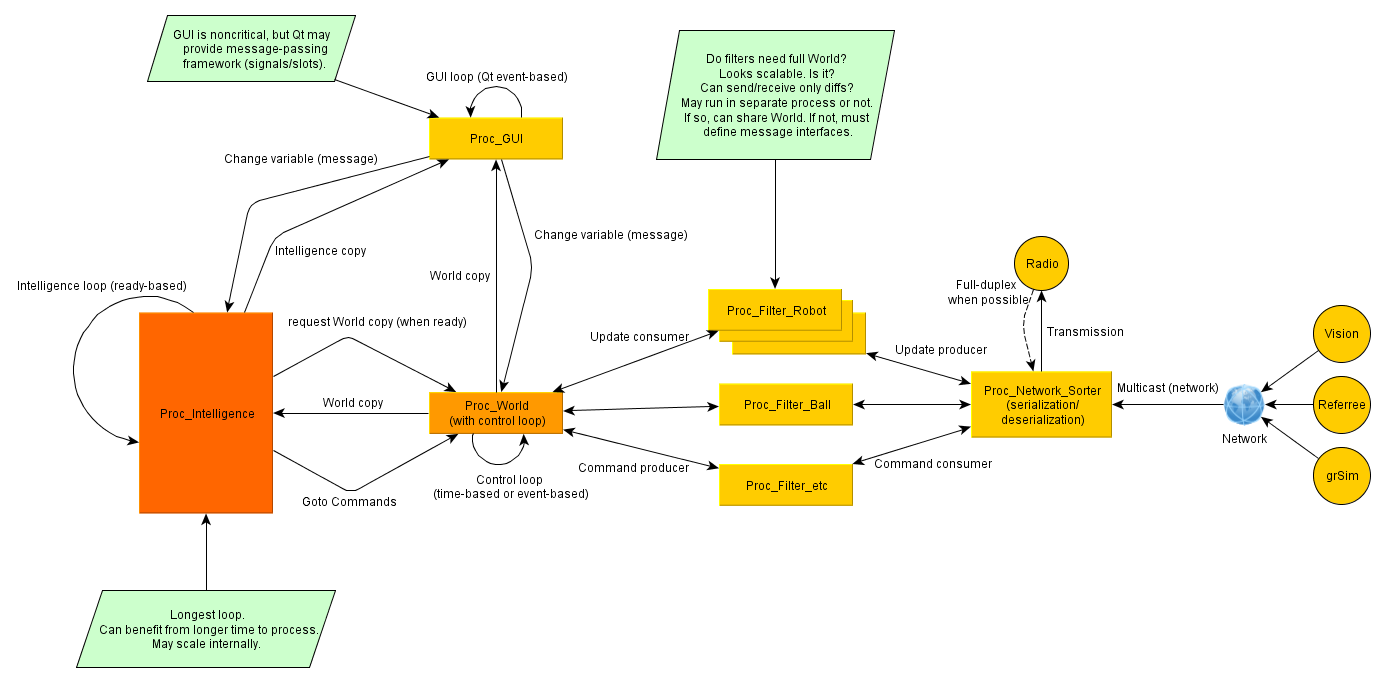
\includegraphics[width = \linewidth]{software-model}
%     \caption{Block diagram of the AI software}
%     \label{fluxogramSoftware}
%\end{figure}
%\end{landscape}

\subsection{Support systems}

The graphical client, ssl-webclient, is a Web interface implemented in nodejs
using WebSockets, HTML5, SVG and ZeroMQ\@.
It has the following functionality: displaying and altering the AI state,
broadcasting games through the internet and playing log files.

Lastly the simulator, grSim, originally developed by Parsian Robotic, was
customized to fit our needs.
It provides the following functionality: simulating the game environment and
exposing an ssl-vision compliant protocol.

\begin{figure}[H]
     \centering
     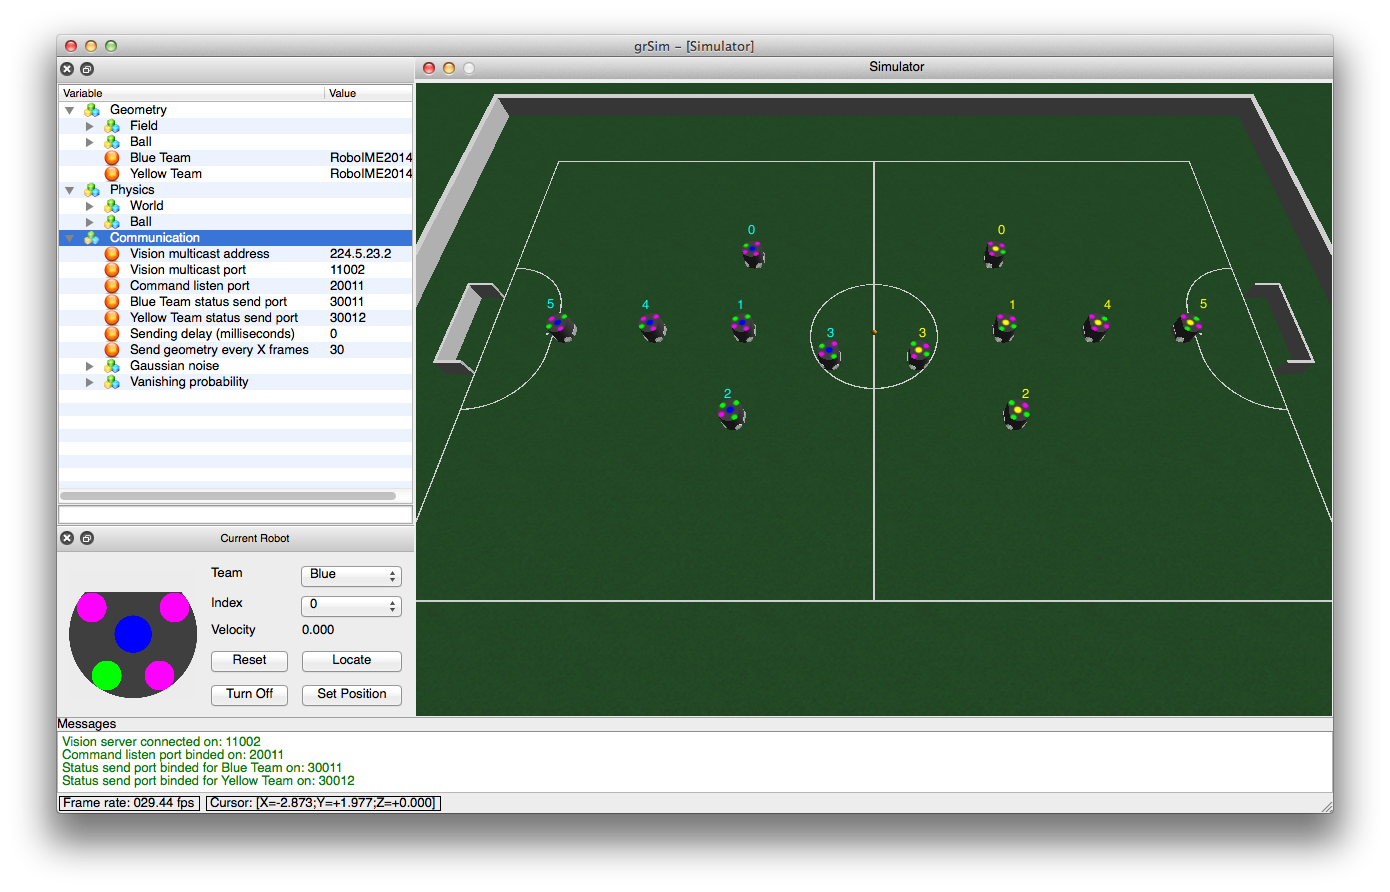
\includegraphics[width = \linewidth]{grsim}
     \caption{Snapshot of the simulator}
     \label{fig:grsim}
\end{figure}

\subsection{Source}

All of the projects above have been open sourced with GPL-like license, with
the main difference being that a derived work used on a competition must have
its source released by the next edition of that competition. The sources of
those projects are available on the team's github page:
\url{http://github.com/roboime/}.

% vim: tw=79 et sw=4 ts=4 filetype=tex
